\subsection{Mobile Application}
This sub-section describes the design of the OpenWRT remote access mobile application. Since this is a proof of concept, we only designed and implemented the application on Android platform.

\subsubsection{Architecture}
Figure \ref{android-architecture} shows the architecture of the Android OpenWRT remote access mobile application. It mainly contains four sub modules: activity module, network communication module, graphical user interfac module and response result parer module. Among these four modules, activities combine the other three modules together to present result to users and take users' inputs.
	\begin{figure*}
		\centering
		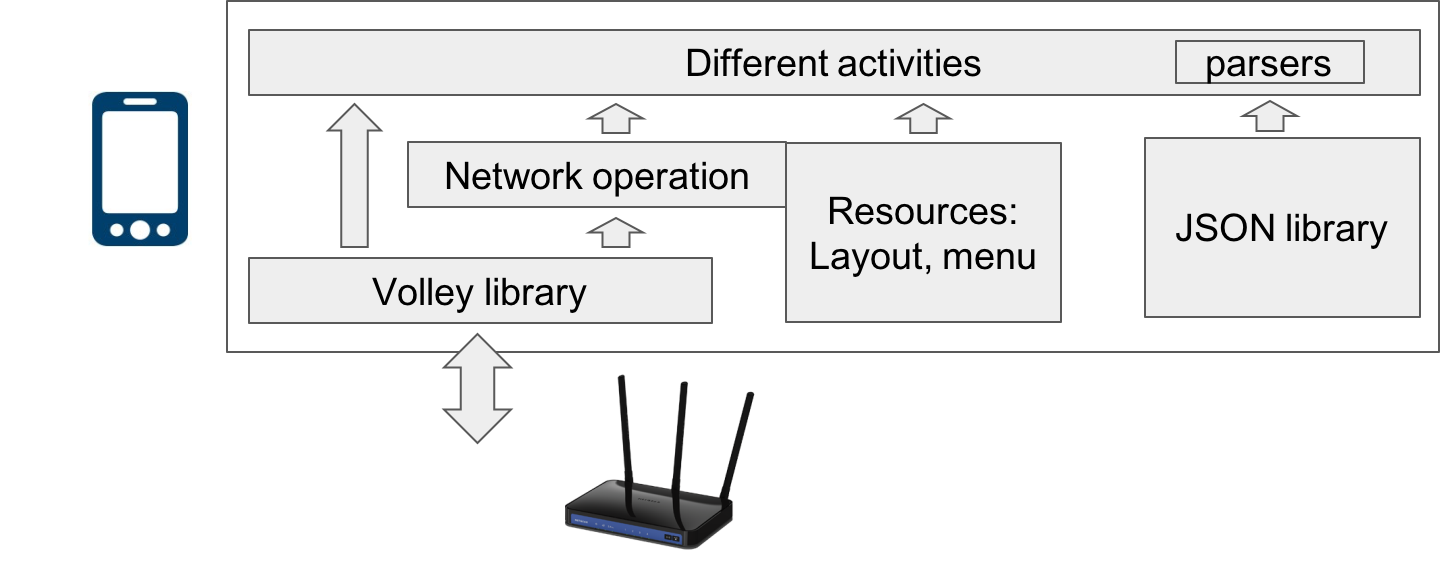
\includegraphics[width=0.75\textwidth]{android-architecture.png}
		\caption{Android Application Architecture}
		\label{android-architecture}
	\end{figure*}

\subsubsection{Network Communication}
Since the application needs to communicate with OpenWRT backend server, it's necessary to provide a network communication module to handle all the network operation, so that other modules can simply use its APIs without worrying about the details.

LuCI backend and application specific traffic analysis backend both provide http-based interfaces. To commuicate with these two backends, the network communication module needs to be able to send ``http POST'' and ``http GET'' requests and receives responses. A key part is to build proper URLs according to backends' requirments. The only difference between ``http POST'' and ``http GET'' is that ``http POST'' carries some parameters in the URL. For example, a ``http POST'' request to communicate with LuCI backend is ``http://<IP address of the OpenWrt Box>:<server port>/cgi-bin/luci/;stok=<stok id>''; a ``http GET'' request to communicate with application specific traffic analysis backend is ``http://<IP address of the OpenWrt Box>:<server port>/output.txt''

\subsubsection{Graphical User Interface}
The goal of the graphical user interface design was to simplify the user interface on a smartphone. To that end, the limitations of the LuCI web interface were studied to provide design guidelines. The first issue analyzed was that LuCI had an issue in its navigation on smartphones. To navigate through the application categories, the user needed to select a category in the navigation menu, then select a subcategory from the dropdown menu. Additionally, changing subcategories within the same category still required selecting the overarching category again. Therefore, a design goal of the application would be to maintain the current category and simply swap subcategories.
	
Another LuCI WebView issue was that unsaved changes would be tracked in a session until committed. Tracking unsaved changes on a web browser can result in session complications, depending on browser settings for caching. Furthermore, the WebView relied on in-browser scripting to provide functional elements, which is a dependency that can be optimized. Therefore another aspect of our design was to make all actions atomic and contained to the screen they are accessed on, to avoid carrying changes. To make all actions atomic, all functional elements in the original WebView would be rebuilt natively in Android.
	
Based on the LuCI framework, the designed Android application's user interface screens consisted of a login screen, then three major categories: status, network, and system. Each category then presented a subnavigation menu that persisted until another major category was selected, allowing users to move more freely within same category.
	
Each separate screen in the subcategories of the major categories was designed to maintain discrete actions and information. Rather than having multiple configuration forms and submission buttons in the same screen, the screen would be limited to at most one form each, with other forms being accessible on a new screen that is linked to by a list on the current screen.